% ===========================================================================
%  QuantMind — CM3070 Final Project, Preliminary Report
%  Template 4.2: Financial Advisor Bot
%
%  Overleaf-ready. Compiles with pdfLaTeX + BibTeX (run: pdflatex -> bibtex ->
%  pdflatex x2). LaTeX is not yet installed locally; upload this folder to
%  Overleaf, or install a TeX distribution, to build the PDF.
%
%  WORD LIMITS (strict per chapter; 6000 total): Intro 1000, Lit Review 2500,
%  Design 2000, Prototype 1500. Only Chapter 4 is complete so far.
% ===========================================================================
\documentclass[11pt,a4paper]{report}

\usepackage[utf8]{inputenc}
\usepackage[T1]{fontenc}
\usepackage{lmodern}
\usepackage[margin=2.5cm]{geometry}
\usepackage{graphicx}
\usepackage{booktabs}
\usepackage{amsmath}
\usepackage{hyperref}
\usepackage[round]{natbib}   % author-year citations; swap to numeric if preferred
\usepackage{caption}

\hypersetup{colorlinks=true, linkcolor=black, citecolor=black, urlcolor=blue}
\graphicspath{{figures/}}

\title{\textbf{QuantMind}\\[0.4em]
       An Explainable AI Financial Advisor Bot for\\
       Intelligent Active Portfolio Management\\[0.8em]
       \large CM3070 Final Project --- Preliminary Report\\
       \normalsize Project Template 4.2: Financial Advisor Bot}
\author{Maira Farukkh}
\date{\today}

\begin{document}

\maketitle
\tableofcontents

% --- Chapter 1: Introduction (max 1000 words) ------------------------------
% ===========================================================================
%  Chapter 1 — Introduction (max 1000 words)   [PLACEHOLDER — to be written]
%  Source: PPT slide 2 "The Problem" + concept. MUST state Template 4.2.
%  Cover: problem (advice cost, behavioural bias, info overload, black-box AI);
%  the QuantMind concept (RL + NLP/FinBERT + XAI behind a web UI); aims;
%  explicit statement that this project uses Template 4.2 (Financial Advisor Bot).
% ===========================================================================
\chapter{Introduction}
\label{ch:intro}

\textit{[To be written — max 1000 words. Draft from PPT ``The Problem'' slide.
Must explicitly state the project uses Template 4.2, Financial Advisor Bot.]}


% --- Chapter 2: Literature Review (max 2500 words) -------------------------
% ===========================================================================
%  Chapter 2 — Literature Review (max 2500 words)  [PLACEHOLDER]
%  Source: PPT Related Work slides 3-6. Cover & critically compare:
%   1. Robo-advisors (Betterment/Wealthfront) — passive, black-box.
%   2. Deep RL for trading (Mnih 2015; Jiang 2017) — opaque, data-hungry.
%   3. FinBERT / LLM sentiment (Yang 2020; Lopez-Lira & Tang 2023) — no decisions.
%   4. XAI & trust in FinTech (Ribeiro 2016 LIME; Arya 2019; Meske 2022).
%  Aim for 4-6 well-discussed pieces with critical analysis + the gap QuantMind fills.
% ===========================================================================
\chapter{Literature Review}
\label{ch:literature}

\textit{[To be written — max 2500 words. Draft from PPT Related Work slides 3--6;
critically evaluate and draw together the four themes, then state the gap.]}


% --- Chapter 3: Design (max 2000 words) ------------------------------------
% ===========================================================================
%  Chapter 3 — Design (max 2000 words)  [PLACEHOLDER]
%  Source: PPT slides 7-9 (gap table, 3-tier architecture, aims & eval plan).
%  Cover: 3-tier architecture (Data layer -> AI/ML engine -> Web interface);
%  component design (RL agent, FinBERT, SHAP/LIME + LLaMA-3 narration, React UI);
%  the project aims; the evaluation strategy (backtesting metrics + SUS/XAI user
%  study); workplan (the 4 phases). Use diagrams. Relate clearly to Template 4.2.
% ===========================================================================
\chapter{Design}
\label{ch:design}

\textit{[To be written — max 2000 words. Draft from PPT architecture and aims
slides; include an architecture diagram and the evaluation/workplan.]}


% --- Chapter 4: Feature Prototype (max 1500 words) -------------------------
% ===========================================================================
%  Chapter 4 — Feature Prototype  (max 1500 words)
%  QuantMind: Explainable AI Financial Advisor Bot (Template 4.2)
% ===========================================================================
\chapter{Feature Prototype}
\label{ch:prototype}

\section{Scope and rationale}
The single most important and technically demanding feature of QuantMind is its
\emph{decision engine}: the reinforcement-learning (RL) agent that converts noisy
market data into an active, risk-controlled portfolio allocation, together with
the explainability layer that justifies each decision. The remaining components
(sentiment fusion, LLM narration, web front end) are comparatively conventional
engineering. This prototype therefore implements the RL agent and its
explanations end-to-end on real market data, to prove that the hardest part of
the design is feasible. It deliberately excludes the FinBERT and LLaMA modules,
which are revisited in Section~\ref{sec:proto-improve} as planned work.

\section{Implementation}

\subsection{Data and features}
Daily adjusted-close prices for five liquid, sector-diverse S\&P~500 constituents
(AAPL, MSFT, JPM, XOM, JNJ) were obtained via the \texttt{yfinance} API
\cite{yfinance} for 2015--2024 (2{,}515 trading days) and cached locally for
reproducibility. From each price series we engineer seven normalised technical
features per asset: 1- and 5-day log returns, a scaled 14-day RSI, a
volatility-scaled MACD histogram, 20-day realised volatility, and two
moving-average ratios (price/SMA-20 and SMA-5/SMA-20). These span the three
classic signal families---momentum, mean-reversion and trend---used in
quantitative trading. The series is split chronologically: 2015--2021 (1{,}743
days) for training and 2022--2024 (752 unseen days) for testing, a deliberately
demanding hold-out spanning the 2022 bear market and the 2023--24 recovery.

\subsection{Environment: portfolio management as an MDP}
Following the deep-RL portfolio-management formulation of Jiang et
al.~\cite{jiang2017}, we model active management as a Markov Decision Process and
implement it as a custom \texttt{Gymnasium} environment. At the close of day $t$
the agent observes the feature vector for all assets plus its current weights;
its action is a real vector that a softmax maps to target weights over the five
assets and cash. A 40\% per-asset \emph{concentration cap} is then enforced
(excess weight redistributed across the remaining assets), encoding a standard
institutional risk constraint and forcing genuine diversification rather than a
single bet. Crucially, a decision taken at day $t$ earns the realised return from
$t\!\to\!t\!+\!1$, so no future information leaks into the state. The reward is
the net log return minus risk and churn penalties:
\begin{equation}
r_t = \log\!\big(1 + R_t^{\text{net}}\big) - \lambda_{\text{risk}}\,\sigma_t
      - \lambda_{\text{turn}}\,\tau_t,
\label{eq:reward}
\end{equation}
where $R_t^{\text{net}}$ is the portfolio return net of a 0.1\% proportional
transaction cost, $\sigma_t$ is rolling 20-day volatility, $\tau_t$ is turnover,
and $\lambda_{\text{risk}}=0.15$, $\lambda_{\text{turn}}=0.02$.

\subsection{Agent}
The policy is trained with Proximal Policy Optimisation (PPO)
\cite{schulman2017}, a robust on-policy actor--critic method well suited to the
continuous action space, via Stable-Baselines3 \cite{sb3} (multilayer-perceptron
policy, two hidden layers of 128 units, 150{,}000 environment steps, fixed seed
for reproducibility).

\subsection{Explainability}
\label{sec:proto-xai}
To make each allocation interpretable we treat the trained policy as a function
$f:\text{observation}\!\to\!\text{weights}$ and attribute its output to the input
features using \emph{Shapley-value sampling} \cite{strumbelj2014}---the
model-agnostic estimator that underlies SHAP \cite{lundberg2017} and generalises
the local-explanation idea of LIME \cite{ribeiro2016}. For each feature $i$ the
Shapley value is the average marginal change in the output as $i$ joins a random
coalition, with absent features drawn from a background distribution; by
construction the attributions sum to $f(x)-f(\text{baseline})$. The algorithm is
implemented from scratch in NumPy (no \texttt{shap}/\texttt{numba} dependency),
keeping the prototype lightweight and the method fully transparent. It produces
both a global feature-importance ranking and a per-decision, plain-English
rationale---the QuantMind explanation a non-technical user would read.

\section{Evaluation}

\subsection{Methodology}
Evaluation follows accepted practice in quantitative finance rather than raw
accuracy. On the unseen test period we report cumulative and annualised return
(CAGR), annualised volatility, the Sharpe \cite{sharpe1966} and Sortino
\cite{sortino1994} ratios, and maximum drawdown, benchmarked against two
references: an equal-weight, drifting \emph{buy-and-hold} portfolio (the standard
passive baseline) and the \emph{best single asset chosen with hindsight} (an
optimistic, non-investable upper bound). All baselines earn the same
realised-return days as the agent.

\subsection{Results}
\begin{table}[h]
\centering
\caption{Held-out test performance (2022-01 to 2024-12, 752 days).}
\label{tab:proto-results}
\begin{tabular}{lcccccc}
\toprule
Strategy & Tot.\ Ret. & CAGR & Vol. & Sharpe & Sortino & Max DD \\
\midrule
\textbf{QuantMind PPO} & \textbf{49.4\%} & \textbf{14.4\%} & 16.2\% & \textbf{0.91} & \textbf{1.34} & $-13.8\%$ \\
Buy \& Hold (1/N)      & 42.0\% & 12.5\% & 16.0\% & 0.82 & 1.20 & $-12.8\%$ \\
Best asset (ex-post)   & 85.1\% & 22.9\% & 27.2\% & 0.89 & 1.35 & $-20.5\%$ \\
\bottomrule
\end{tabular}
\end{table}

Table~\ref{tab:proto-results} shows the agent achieves a higher Sharpe ratio
(0.91 vs.\ 0.82), Sortino ratio, CAGR and total return than buy-and-hold at
essentially the same volatility, and even exceeds the hindsight best-single-asset
Sharpe while incurring far smaller drawdown (-13.8\% vs.\ -20.5\%). The equity
curve (Fig.~\ref{fig:proto-equity}) confirms the agent tracks above the passive
baseline throughout the test window. The allocation plot
(Fig.~\ref{fig:proto-alloc}) demonstrates genuine \emph{active} management: the
agent rotates from an energy (XOM) overweight during the 2022 inflation shock
toward financials and healthcare later, always within the 40\% cap, at a moderate
4.8\% average daily turnover. The Shapley analysis
(Fig.~\ref{fig:proto-shap}) reveals the decision logic: allocations are driven
most by position inertia (current weights---consistent with the churn penalty),
followed by MACD trend strength and RSI signals. A representative generated
rationale reads: \emph{``QuantMind allocates most to JNJ (40\%); main drivers:
its RSI and price-vs-20-day-average increased the weight.''}

\begin{figure}[h]
\centering
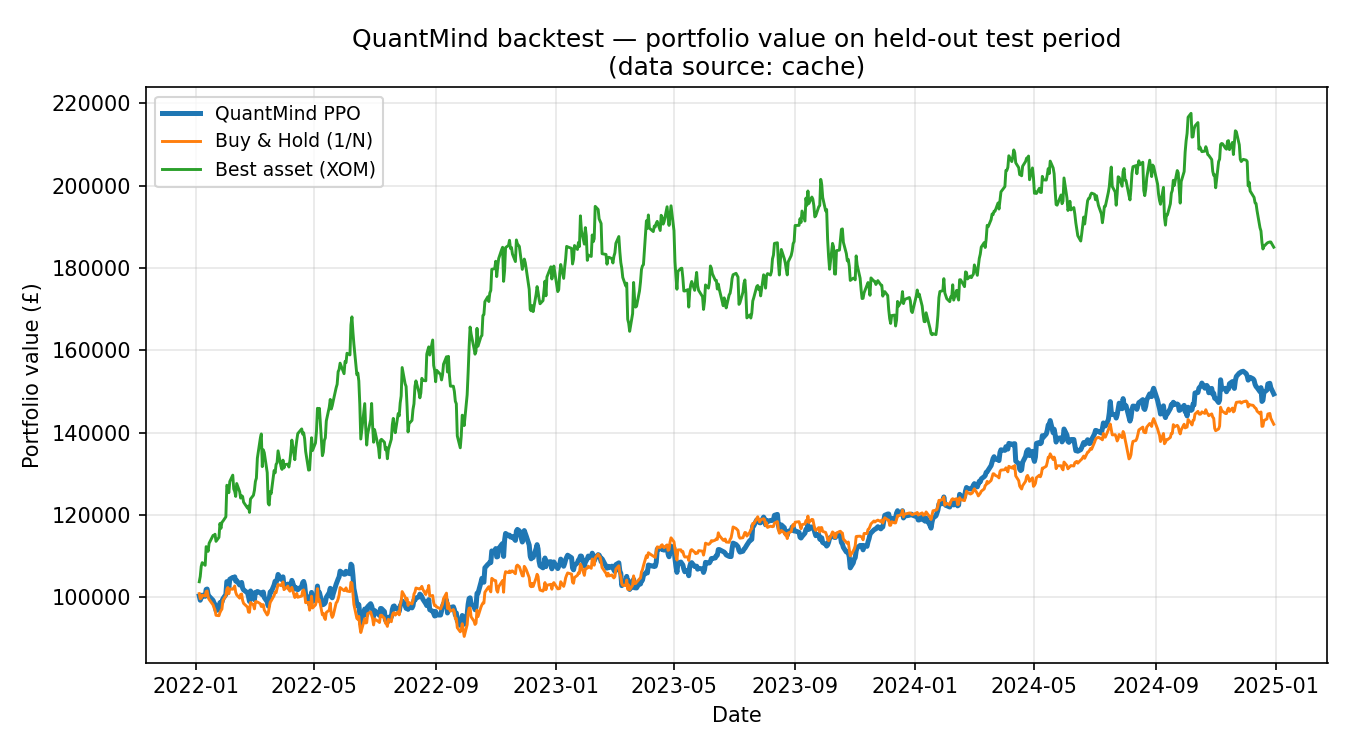
\includegraphics[width=0.92\textwidth]{figures/equity_curve.png}
\caption{Portfolio value over the held-out test period.}
\label{fig:proto-equity}
\end{figure}

\begin{figure}[h]
\centering
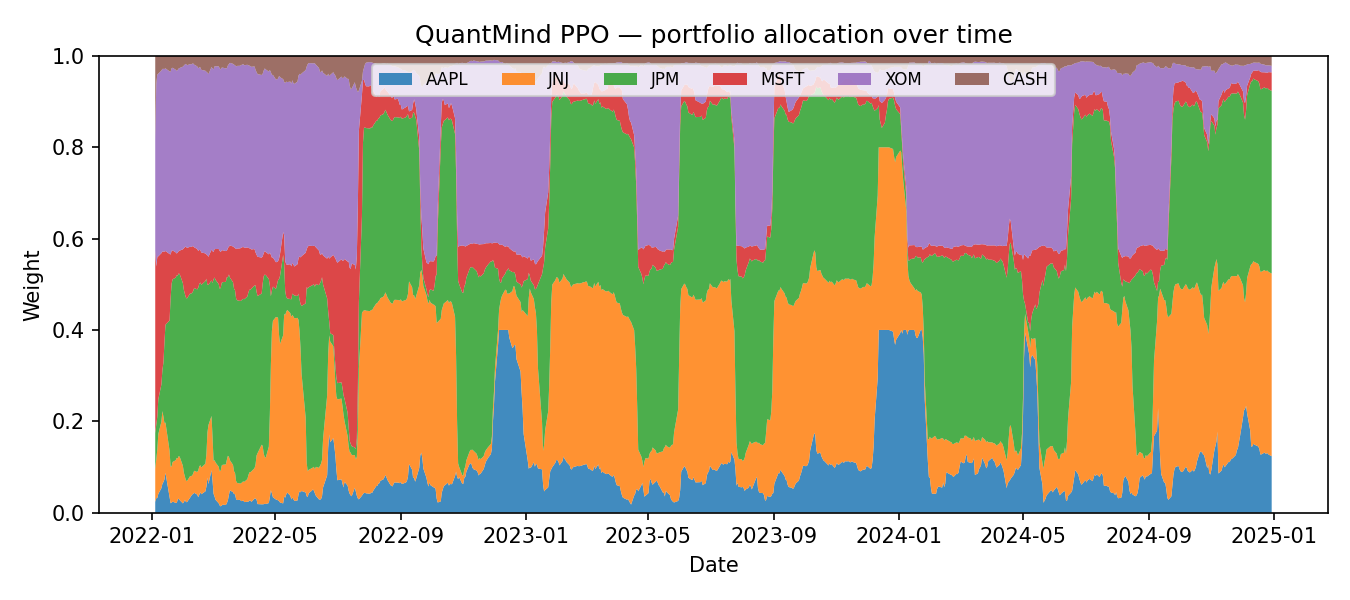
\includegraphics[width=0.92\textwidth]{figures/allocation.png}
\caption{Agent allocation over time, showing active rotation under the 40\% cap.}
\label{fig:proto-alloc}
\end{figure}

\begin{figure}[h]
\centering

\includegraphics[width=0.7\textwidth]{figures/shap_importance.png}
\caption{Global feature importance (mean $|$Shapley value$|$) over test decisions.}
\label{fig:proto-shap}
\end{figure}

\subsection{Critical evaluation}
The prototype validates the core hypothesis: an RL agent can learn a stable,
diversified, risk-aware active strategy that beats a passive baseline on
risk-adjusted terms out-of-sample, and its decisions can be explained
quantitatively. Building it also surfaced two important lessons. First, an early
version produced an implausible Sharpe of 8.5; investigation revealed
\emph{lookahead bias}---the reward used the same day's return the agent could
already observe---which was corrected, underscoring the need for careful temporal
hygiene in financial RL. Second, an unconstrained reward led the agent to
\emph{overtrade} (daily turnover of 16\%), eroding returns through costs; adding
the turnover penalty and concentration cap of Eq.~\ref{eq:reward} produced the
disciplined behaviour reported here. Limitations remain: a Sharpe of 0.91 falls
short of the project's aspirational 1.2 target; results rest on a single asset
universe, a single test period and one random seed; and the agent's edge is
modest and may be regime-dependent.

\subsection{Planned improvements}
\label{sec:proto-improve}
Several concrete steps follow directly. \emph{Robustness:} walk-forward
(rolling-origin) validation and multi-seed averaging to quantify variance.
\emph{Signal:} fusing the FinBERT news-sentiment feature from the design into the
state, the prototype's most promising untested lever. \emph{Objective:} a
differential-Sharpe reward \cite{moody2001} to optimise risk-adjustment directly.
\emph{Trust:} the planned user study evaluating whether the Shapley-based
explanations measurably increase non-expert confidence, closing the loop with the
explainability literature.


% --- References ------------------------------------------------------------
\bibliographystyle{plainnat}
\bibliography{references}

\end{document}
